\chapter{Proxy RouteFlow em Java}

\section{Introdução aos Proxies RouteFlow (RFProxy)}

Nos capítulo à respeito do projeto RouteFlow foi dado
uma visão geral de todos os três módulos usados para
construir o projeto. Esse capitulo se foca principal no 
módulo proxy, desenvolvido como foco principal do trabalho de
conclusão de curso.

Como já dito nos capítulos anteriores, o proxy RouteFlow ou
RFProxy atua como um tradutor de protocolos, convertendo
mensagens no protocolo RouteFlow para o protocolo OpenFlow
e vice-versa. Todos os eventos do ambiente físico são notificados
ao servidor na forma de mensagens, sendo as mesmas tratadas 
e processadas de acordo com o evento. Cada evento gera uma 
ação ao servidor (RFServer), que responde na forma de uma 
mensagem ao proxy (RFProxy), instruindo-o a tomar certa atitude.
Dentro dessas atitudes estão a criação das regras nos \textit{
switches OpenFlow}, fazendo toda a rede física se comportar
da maneira proposta pelo ambiente virtual e seus algoritmos de
roteamento.

As mensagens do protocolo RouteFlow, como já citado nos
capítulos anteriores, vem via o mecanismo de troca de mensagens
entre processos (IPC) implementado através do banco de dados
centralizado. Tal característica força o desenvolvedor escolher
as linguagens de programação com suporte à manipulação do
banco de dados usado pelo projeto RouteFlow, que no caso
é o MongoDB.

As mensagens do protocolo \textit{OpenFlow} são advindas do ambiente
físico e necessitam de algum mecanismo de captura e processamento.
Tal mecanismo é provido pelos softwares de controle \textit{
OpenFlow}. Dentre os diversos disponíveis, os mais famosos
são o NOX, o POX e o Floodlight. Todos os controladores
\textit{OpenFlow} são operados apenas como 
interfaces de programação, provendo todas as funções de captura
de eventos e criação de mensagens do protocolo \textit{OpenFlow}.

Cada um dos controladores citados acima foi desenvolvido em
uma linguagem de programação diferente, forçando o desenvolvedor
a trabalhar na mesma linguagem do controlador de forma a 
opera-lo como forma de interface de programação (API). 
Cada controlador possui vantagens exclusivas, tendo sido construídos
com propósitos diferentes. O controlador NOX se destaca pela
performance, pelo fato de ser construído em C++ e possui
código compilado. O controlador POX se destaca pela
facilidade de programação provida pela linguagem Python mas
possui desempenho inferior devido ao fato do Python ser
interpretado. 

O controlador escolhido para uso neste trabalho foi 
o Floodlight. Sendo desenvolvido para ser usado
principalmente por  administradores de rede, possui uma 
série de aplicações nativas que permitem o seu controle
via aplicações externas. Uma dessas aplicações nativas 
permite a recepção de mensagens via mensagens REST,
possibilitando ao desenvolvedor manipular sua rede sem
a necessidade de programar um módulo dedicado. Tal fato
dificultou o desenvolvimento do trabalho, visto que grande 
parte da documentação disponível para consulta era voltada
apenas para os administradores, sem levar em consideração os 
desenvolvedores de aplicações em Java. O fato
de ter sido construído em Java pode impactar em seus desempenho
mas tal impacto é recompensado visto o grande número de 
recursos disponíveis. Um dos recursos que pode ser citado
é a interface gráfica usada para visualização da rede que
no futuro poderá ser adaptada para uso como o projeto 
RouteFlow. A comunidade de usuários é grande e bastante
ativa, fato notado pela grande quantidade de postagens no
fórum oficial do controlador.

Os dois proxies RouteFlow (RFProxy) já existentes durante a 
criação desse trabalho seguem um mesmo algoritmo, o que 
facilita muito o entendimento geral. A maior dificuldade no
desenvolvimento de um novo proxy RouteFlow (RFProxy) são
as características exclusivas de cada linguagem de programação,
cabendo ao desenvolvedor as adaptações necessários para 
implementar o algoritmo. A linguagem Java já possuía uma
ótima API para comunicação com o banco de dados MongoDB
e para a manipulação de mensagens no protocolo JSON. Um fato
que trouxe certa dificuldade no trabalho foi o desenvolvimento
de uma aplicação com múltiplas threads em Java. 

A Figura \ref{fig:esquematicoProxy} ilustra de forma simples as
funções básicas bem como a direção das informações tratadas
pelo proxy RouteFlow (RFProxy). É interessante notar que o 
proxy só se comunica com com o restante do ambiente através
do mecanismo de troca mensagens entre processos (IPC) basedo
no banco de dados centralizado.
\newline
\newline
\newline
\newline


\begin{figure}[h] 
\centering
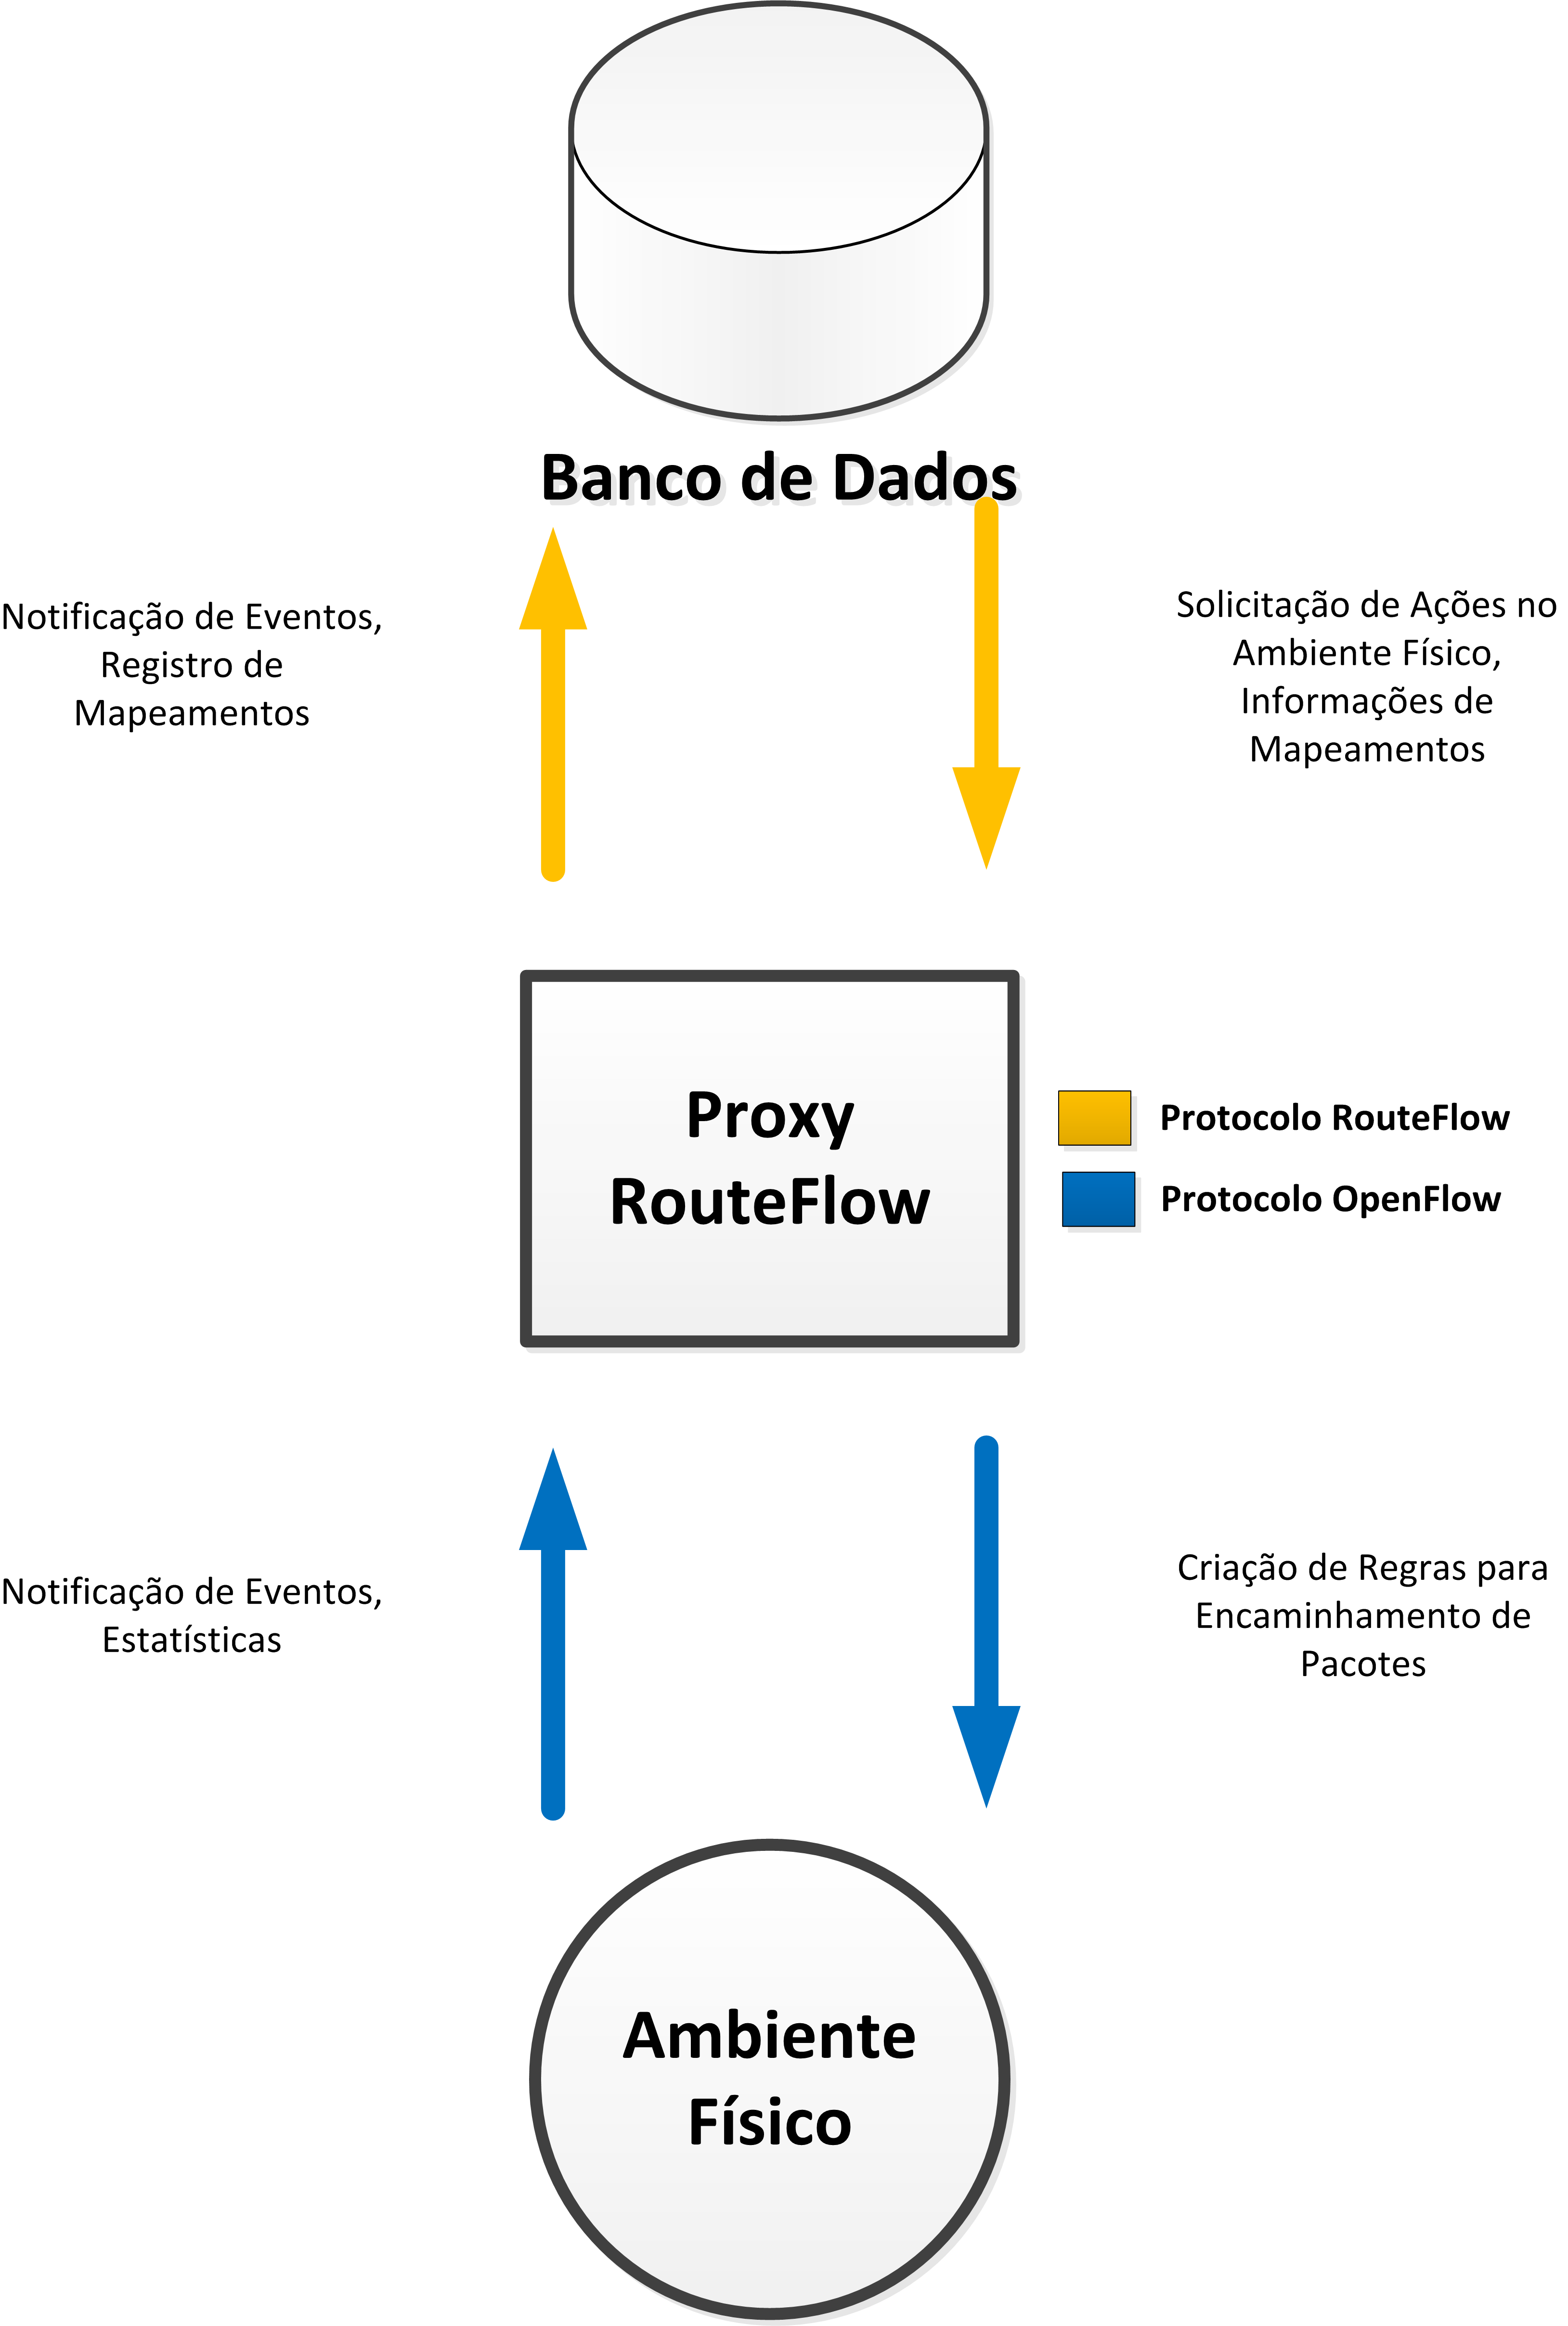
\includegraphics[width=120mm]{esquematico_geral_proxy.png}
\caption{Esquema Geral do Proxy RouteFlow (RFProxy).}
\label{fig:esquematicoProxy} 
\end{figure}
 

\section{Descrição Geral da Estrutura do Proxy RouteFlow em Java}

Todos os componentes do proxy RouteFlow em Java foram agrupados em classes. O agrupamento em classes 
facilita a 
organização geral do código bem como a sua futura manutenção. Abaixo temos os componentes do proxy com 
suas respecitivas descrições:

\begin{itemize}
\item \textit{MongoIPCMessageService:} Responsável pela
 comunicação entre o servidor RouteFlow e o proxy 
RouteFlow. A arquitetura básica do projeto RouteFlow 
faz uso de um banco de dados não SQL para troca de 
mensagens entre seus componentes, sendo que o banco 
de dados escolhido foi o MongoDB. 

O MongoDB possui 
alto desempenho sendo totalmente escrito em C++, outro
 aspecto importante é o fato de não ser SQL, o 
que facilita a sua integração com as  principais linguagens
 de programação. 
O RouteFlow cria inúmeras tabelas no banco de dados, cada uma 
responsável pela comunicação entre um par 
de componentes, como toda comunicação é feita através de um 
sistema de banco de dados é possível que a 
comunicação entre componentes seja feita de forma simples, sem 
nenhum vinculo com a linguagem de 
implementação do mesmo. 

O componente MongoIPCMessageService 
cria um IPC (Inter-Process Communication) 
entre o servidor RouteFlow e o proxy RouteFlow. Os comandos são 
enviados de um componente para o outro 
na forma de mensagens pré-definidas. Cada mensagem define uma 
ação à ser tomada em relação aos eventos 
que vão ocorrendo ao longo da execução do ambiente. No corpo da 
mensagem estão os parâmetros que 
deverão ser usados para tomada da ação. Todas as mensagens que 
são colocadas na tabela pelo servidor RouteFlow 
possuem um campo que indica se a mesma já foi tratada e em caso 
negativo cabe ao proxy tomar a ação e 
atualizar o campo da mensagem. Para tratamento das mensagens é 
gerado uma thread em looping infinito 
cujo único proposito de existência é o tratamento de novas mensagens. 
Essa característica pretende ser melhorada nas próximas versões 
do RouteFlow;
\item \textit{RFProtocolFactory:} Responsável pela criação das 
mensagens do protocolo RouteFlow. Cada 
tipo de mensagem RouteFlow é representada por um código e 
por uma respectiva classe. É papel do 
RFProtocolFactory retornar os objetos de mensagens à partir de 
seu código. Esta estrutura facilita a 
inserção de novas mensagens no ambiente evitando a reprogramação 
de outras classes;
\item \textit{RFProtocolProcessor:} Responsável pelo processamento 
de mensagens vindas do servidor 
RouteFlow. Este componente define o como será tratada cada mensagem 
vinda do servidor RouteFlow. As 
mensagens são lidas através do IPC e repassadas para tratamento.
\item \textit{AssociationTable:} Tabela mantida pelo proxy para armazenar 
a associação entre portas no 
ambiente virtual e porta no ambiente físico.
\end{itemize} 

\section{Descrição das Mensagens Traduzidas pelo Proxy RouteFlow}

\begin{itemize}
\item \textit{PortRegister}
\item \textit{PortConfig}
\item \textit{DatapathConfig}
\item \textit{RouteInfo}
\item \textit{FlowMod:} Mensagem utilizada para 
solicitação da instalação de regras nos switches 
OpenFlow. As mensagens FlowMod possuem em seu 
corpo um conjunto de parâmetros que define uma nova regra 
a ser aplicada à um switch OpenFlow. Cabe ao proxy 
criar a regra e envia-la corretamente ao switch. 
Para envio das regras é necessário a manipulação do 
protocolo OpenFlow. O Floodlight fornece uma série de 
funções para esse proposito, sendo usado como uma 
API de comunicação entre os switches OpenFlow e o 
proxy.
\item \textit{DatapathPortRegister:} Mensagem utilizada 
para registrar as portas dos switches OpenFlow 
no servidor RouteFlow. Esse registro é feito para que cada 
porta seja associada à uma porta da máquina 
virtual do ambiente virtual.
\item \textit{DatapathDown:} Mensagem utilizada para que 
o proxy informe ao servidor RouteFlow sobre a 
desconexão de um switch OpenFlow. O Floodlight, no papel 
de controlador OpenFlow, mantem um conjunto de 
informações à respeito dos switches OpenFlow ativos, 
podendo detectar quedas nas conexões dos mesmos. O 
servidor RouteFlow necessita ter esse tipo de informação para 
possíveis alterações nas regras dos 
switches OpenFlow.
\item \textit{VirtualPlaneMap:} Mensagem utilizada para que 
o proxy associa cada porta do switch 
OpenFlow à uma porta de uma máquina virtual no ambiente 
virtual.
\item \textit{DataPlaneMap:} Mensagem utilizada para que o 
servidor RouteFlow informe ao proxy à 
respeito de uma associação de porta bem sucedida. O proxy 
mantém uma tabela de associação entre portas 
no ambiente virtual e portas no ambiente físico.
\end{itemize}

